


\titleformat
{\chapter} % command
[display] % shape
{\bfseries\Large\itshape} % format
{Capítulo \ \thechapter} % label
{0.5ex} % sep
{
    \rule{\textwidth}{1pt}
    \vspace{1ex}
    \centering
} % before-code
[
\vspace{-0.5ex}%
\rule{\textwidth}{0.3pt}
] % after-code


\chapter{Planteamiento del Problema}


\section*{Introducción al Problema}
\addcontentsline{toc}{section}{Introducción}
La salud mental se ha convertido en una de las crisis sanitarias más críticas del siglo XXI. De acuerdo con la Organización Mundial de la Salud (OMS) \cite{chatzaki2025overview}, 
fenómenos recientes como la pandemia global desencadenaron un aumento del 25\% en la prevalencia de la ansiedad y la depresión a nivel mundial.

El estres es capaz de afectar condiciones quimicas cerebrales mediante la hormona del cortisol, afectando capacidades de resolución de problemas y toma de deciciones
incremento de la presión sanguínea y otras condiciones mentales y fisiologicas aun en estudio con un indicador relacionado a estres \cite{gopi2024serenepulse}.
Desde la época pandemica, la necesidad de diagnóstico remoto aumento considerablemente emergiendo en técnicas que permitan el los procesos a distancia \cite{transphys2023}.
Ante esta urgencia, la fotopletismografía remota (rPPG) ha emergido como una tecnología prometedora para el monitoreo no invasivo de signos vitales sin necesidad de contacto fisico \cite{casado2024design}, 
permitiendo extraer la Variabilidad de la Frecuencia Cardíaca (HRV) a través de cámaras de video para diagnosticar el estrés de manera automatizada \cite{fontes2024enhancing}. \\

Sin embargo extraer está información (HRV) requiere del uso de sensores los cuales pueden ser intrusivos o no intrusivos. Para ciertos aspectos el uso de sensores
intrusivos puede traer inconvenientes para las personas dado los factorees de poca portabilidad del sensor, espacios especializados, personas que tienen alguna
condición que no les permite el uso prolongado de estos sistemas entre otros \cite{clinical2026software}. Es un problema que el uso de sensores no intrusivos (rPPG)
ha venido a solucionar pero llevando así mismo sus propios retos. Dichos retos incluyen el debilitamiento de la señal pletismográfica por la baja reflectancia de la hemoglobina 
en condiciones de iluminación reducida, donde no siempre el espacio permite una iluminación perfecta generando así una baja calidad en la información obtenida \cite{liang2023selfadaptive}.\\


El siguiente es el diagrama del árbol de problemas (\ref{fig:arbol_de_problemas}), el cual contiene el problema principal, las causas y los efectos derivados de este:

\begin{center}
\begin{figure}[h]
            \centering
            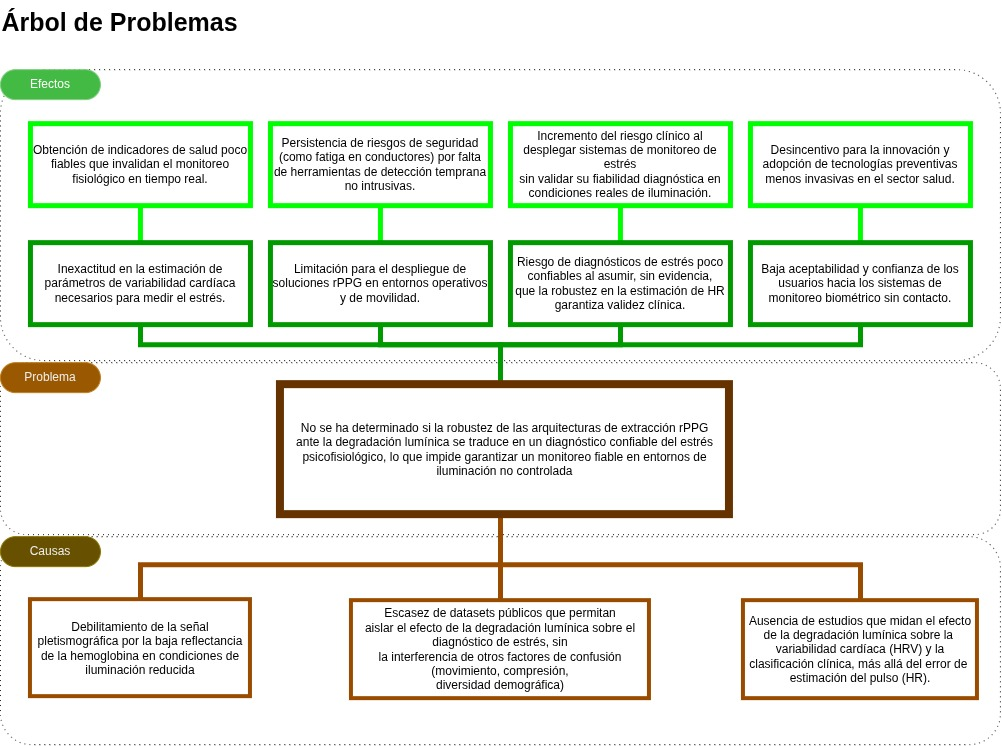
\includegraphics[scale=0.44]{images/arbol_de_problemas.jpg}
            \caption{Árbol de problemas} 
            \label{fig:arbol_de_problemas}
        \end{figure}
\end{center}

\section{Análisis del Problema}

\begin{itemize}
    \item \textbf{Debilitamiento de la señal del pulso por falta de luz en la piel} Para que las cámaras puedan medir el pulso a distancia, es necesario que la 
    luz rebote en los vasos sanguíneos del rostro y regrese al sensor. Sin embargo, cuando la iluminación es muy baja, este rebote es casi imperceptible. En sus 
    experimentos con iluminación controlada, Z. Yang, H. Wang y sus colaboradores demostraron que, al bajar la luz a niveles mínimos, la señal útil proveniente 
    de la sangre prácticamente desaparece de la piel \cite{yang2022image_en}. En ese punto, la cámara deja de captar cambios de color y comienza a registrar 
    únicamente su propio ruido electrónico, lo que genera errores críticos en las fórmulas de medición tradicionales.

    \item \textbf{Escasez de bases de datos relacionadas con estrés diversas y realistas para entrenar a la IA} Para que los sistemas de Inteligencia Artificial funcionen en la vida 
    diaria, necesitan aprender de videos que incluyan a personas muy distintas bajo condiciones de luz cotidianas. No obstante, al analizar 58 bases de datos 
    públicas, Pegueros y Rodríguez-Arce comprobaron que la gran mayoría de las investigaciones utilizan videos grabados en laboratorios con luz controlada, 
    excluyendo a personas de diversos tonos de piel o edades \cite{rodriguez2025datasets}. Aunque algunos investigadores, como Rodrigues y Garcia, han intentado 
    solucionar esto creando conjuntos de datos con luz natural (como rPPG-10), ellos mismos mencionan que las condiciones de población y la variedad de tonos de 
    piel aún no son lo suficientemente amplias \cite{rodriguez2025datasets}. Además de este sesgo, Park et al. señalaron en su estudio que el proceso de validar 
    estos videos con médicos expertos es sumamente costoso, revelando que los registros grabados en escenarios oscuros son prácticamente inexistentes en la 
    comunidad científica \cite{yu2024rgbnir}.

    \item \textbf{Los modelos de extracción de señal rPPG y la condición de oscuridad} 
    
    La extracción de señal de fotopletismografía existe hace mas de 15 años y algunos algoritmos considerados hoy en día como algoritmos tradicionales \cite{yang2022assessment_dl},
    como GREEN, ICA, CHROM, POS y PBV, se fundamentan en principios analíticos, modelos de reflexión óptica de la piel o técnicas de separación 
    ciega de fuentes para aislar la variación del volumen sanguíneo a partir del promediado espacial de canales RGB en regiones de interés (ROI) faciales \cite{yu2023physformer, xu2023ivrrppg, liang2023selfadaptive, wu2026udarppg}. 
    Los algoritmos tradicionales presentan una vulnerabilidad crítica ante condiciones de baja iluminación, ya que la atenuación de la luz reduce la 
    amplitud de la señal pulsátil y provoca que el ruido de cuantización del sensor domine especialmente en los canales rojo y azul, rompiendo los 
    supuestos geométricos y de tono de piel sobre los que se construyen modelos como POS y CHROM \cite{chen2024image_en, xi2022weighted}


    En los últimos años, el campo de la fotopletismografía remota (rPPG) ha migrado de los algoritmos analíticos tradicionales hacia enfoques de aprendizaje 
    profundo orientados a los datos, destacando las redes convolucionales espacio-temporales (2D/3D CNN), los Vision Transformers (ViT) y, más recientemente, 
    los Modelos de Espacio de Estados (SSM / Mamba). A diferencia de las aproximaciones clásicas, estos modelos aprenden de forma automática las 
    representaciones espacio-temporales complejas que conectan las variaciones micro-cromáticas de la piel con la señal fisiológica \cite{debnath2026advanced_signal, chen2024image_en, yang2022assessment_dl}. Para 
    contrarrestar la pérdida de precisión en escenarios de baja iluminación donde el ruido del sensor opaca la fluctuación sanguínea, la literatura 
    reciente ha implementado diversas estrategias: 
    
    \begin{enumerate}
        \item técnicas de aumento de datos por brillo para forzar la invariancia a la luminancia durante el entrenamiento \cite{debnath2026advanced_signal}.
        \item módulos de realce de imagen y compensación de luz (como IEM o LEM) acoplados previa a la extracción \cite{yang2022assessment_dl, kim2022study}.
        \item mecanismos de atención global y complejidad lineal (ViT y Mamba) para preservar la periodicidad del pulso a largo plazo \cite{yang2022assessment_dl, chen2024image_en}.
        \item fusión multimodal (RGB e Infrarrojo Cercano - NIR) junto con paradigmas auto-supervisados \cite{yang2022assessment_dl, speth2023hallucinated}.
    \end{enumerate}

    En el capítulo de estado del arte y metodología se abordarán con mayor profundidad el trabajo de estos algoritmos.



    
    % Al realizar la búsqueda de los modelos consolidados en el campo del rPPG, las 
    % Redes Neuronales Convolucionales (CNN) han sido bastante empleadas para este tipo de tareas. Sin embargo, su dominio se ha forjado en gran parte sobre entornos con 
    % iluminación ideal, y es ahí donde reside la raíz del problema. El inconveniente principal es que una CNN analiza la imagen a través de 
    % filtros locales. Como señala Z. Yu, esta arquitectura se enfoca en parches pequeños de píxeles, lo que le impide entender la cara como un todo 
    % \cite{yu2023physformer}. Cuando aparecen sombras, la red intenta extraer señales de zonas oscurecidas y acaba perdiendo el rastro del pulso. Investigaciones 
    % dirigidas por S. Chen han demostrado que, en niveles de iluminación muy bajos, el rendimiento de estas redes cae drásticamente, ya que 
    % son incapaces de distinguir entre las micro-variaciones reales de la sangre y la región visual del video \cite{chen2024image_en}. A esto se suma la 
    % advertencia de B. Acharya \cite{acharya2025reliability}, quien destaca que la fiabilidad de estos modelos se rompe en escenarios de baja visibilidad, donde 
    % la IA no puede decidir qué partes del rostro son confiables y cuáles no, procesando sombras como si fueran datos válidos.

    

    %AgregadoSep2026
    % \item \textbf{La solución híbrida (CNN 3D + ViT) como arquitectura resiliente} 
    % Frente a las limitaciones de ambas aproximaciones, sería ideal e incluso la literatura reciente resalta la necesidad de integrar una arquitectura híbrida que 
    % combine las fortalezas de los modelos convolucionales y los modelos basados en atención. Por un lado, la inclusión de un módulo inicial convolucional 
    % 3D (\textit{Stem}) aporta el sesgo inductivo espacial necesario para extraer características cromáticas locales de la piel y estabilizar el 
    % entrenamiento. Por otro lado, la integración posterior de un Vision Transformer permite modelar dependencias espacio-temporales a largo plazo y 
    % filtrar las fluctuaciones globales causadas por la escasez de iluminación. Como destacan R. Wang, H. Sun y otros. \cite{transphys2023}, emplear un \textit{Stem} 
    % convolucional en lugar de una partición directa de parches de Transformer hace que el entrenamiento sea más estable y permite construir extractores de 
    % características con atención a la estructura local y contexto global de ambas.

\end{itemize}

\section{Formulación del problema}
%ModificadoSEP2026
¿En qué medida la degradación lumínica compromete la clasificación de estrés psicofisiológico
a través de la señal fisiológica rPPG?


